\section{Technischer Bericht}

\subsection{Einleitung und Übersicht}
Da diese Bachelorarbeit auf der Studienarbeit ''Methode 635 als Cross Plattform App mit Xamarin'' \cite{methode635-sa} aufbaut, wird an einzelnen Stellen in diesem technischen Bericht auf die Studienarbeit verwiesen. Auch wird davon ausgegangen, dass dem Leser Begriffe wie ''Methode 635'' oder ''Xamarin'' bereits geläufig sind. Ist dies nicht der Fall, können allfällige Wissenslücken in diesen Bereichen in der erwähnten Studienarbeit nachgelesen werden.

Der technische Bericht selbst besteht neben diesem Kapitel noch aus sieben weiteren Unterkapiteln. 

Auch hier führten wir zunächst eine Vorstudie durch, in der wir grundsätzliche Analysen durchführten und Fragen klärten. Dabei ging es vor allem um die Frage, wie Dateien in einer Datenbank gespeichert werden können. All dies ist im Kapitel ''Vorstudie'' niedergeschrieben.
Im Kapitel der ''Anforderungsspezifikation'' listen wir alle funktionalen sowie nicht-funktionalen Anforderungen auf, welche neu dazu kamen. Das Domain-Modell findet sich im Kapitel ''Domainanalyse''.

Die ''Architektur\-dokumentation'' ist das nächste Kapitel und dokumentiert die logische Architektur, sowie das Deployment. Jegliche Entscheidungen, welche wir in Bezug auf die Architektur getroffen haben, werden im Kapitel ''Architekturentscheide'' begründet.

Während der gesamten Umsetzung der Applikation sind natürlich auch Probleme aufgetreten. Diese haben wir im Kapitel ''Herausforderungen'' zusammengetragen.

Die eigentliche Implementation haben wir im Kapitel ''Ergebnisse'' dokumentiert.

Zum Schluss blicken wir im Kapitel ''Schlussfolgerungen'' nochmals kritisch auf unser Projekt zurück und bewerten unsere Arbeit und geben einen Ausblick, wie man die Applikation noch erweitern könnte.




\subsection{Vorstudie}
Dieser Abschnitt dokumentiert die Vorarbeiten in verschiedenen Bereichen, die für das Abwickeln dieses Projektes relevant sein können. Dabei werden die entsprechenden Themen analysiert und es wird abgewägt, inwiefern diese für den Projekterfolg von Nutzen sein können. Stellt sich heraus, dass eines der analysierten Themen sinnvoll und machbar ist, wird es in das Projekt integriert.
\subsubsection{Solution Strategy}

In der von Gernot Starke entwickelten Vorlage zur Software Architektur Dokumentation arc42 \cite{arc-42} sowie in seinem Buch \textit{Effektive Softwarearchitekturen} \cite{eswa}, befindet sich ein für uns besonders interessanten Abschnitt namens \textit{Solution Strategy}. Darin ist ein Vorschlag angeboten, wie man in der Synthese der Software Architektur die Ansätze zur Lösungsfindung erarbeitet und dokumentiert. Dieser Vorschlag besteht aus mehreren Tipps zum Inhalt, zur Darstellung und zur Entwicklung dieser Ansätze. Als Beispiel beinhaltet dieser Vorschlag folgenden Tipp: ``Erkläre die Lösungsstrategie so kompakt wie möglich (z.B. als Liste von Schlüsselwörtern)``. Da sich dieses Projekt intensiv mit Lösungsfindungsmethoden auseinandersetzt, könnte die Solution Strategy nützlichen Input bieten, wie der Lösungfindungsprozess in unserer Applikation gestaltet werden könnte. 

Eine mögliche Erweiterung unserer Applikation wäre, ein zusätzliches Modul für eine Lösungsfindungsvariante anzubieten. Dabei käme beim Erstellen eines Brainstormingfindings die Auswahl zwischen zwei Typen von Lösungsfindungen: ``Software Architektur Lösung`` und ``Generelle Lösung``. Bei der Software Lösung würden dann die Tipps von arc42 eingearbeitet sein, wobei eine Abbildung gemäss Tabelle \ref{tab:arc42-mapping} vom Kontext des arc42-Templates in den Applikationskontext denkbar wäre.

\renewcommand{\arraystretch}{1.7}
\begin{table}
	\centering
	\begin{tabular}{|p{6cm}|p{6cm}|}
		\hline
		\textbf{arc42 \& eswa\tablefootnote{Buch Effektive Softwarearchitekturen}-Kontext} & \textbf{Applikationskontext}\\
		\hline
		Lösungsansatz finden & Aufgabe von Benutzer, Kreativität ist von Benutzer gefragt\\
		\hline
		Solution Strategy so genau wie möglich erklären (z.B. als Liste von Keywords) & Liste von Keywords mittels Textinput \\
		\hline
		Lösungsansatz als Tabelle beschreiben & Tabellarische Darstellung mithilfe der Skizzenfunktion\\
		\hline
		Lösungsansatz im Kontext der Qualtätsattribute beschreiben & Bezugnahme auf Qualitätsattribute mittels Textinput, oder Auswahlliste mit definierten Qualitätsattribute anbieten\\
		\hline
		Konzepte, Views oder Code referenzieren & Liste von definierten (Microservices-API-)Patterns\cite{microservices-api} als Input anbieten (z.B. \textit{Frontend Integration}, mit Icon und kurzem Beschrieb des Patterns)\\
		\hline
		Lösungsansatz inkrementell und iterativ wachsen lassen & Durch rundenbasiertes Brainwriting gegeben. \\
		\hline
		Lösungsansatz rechtfertigen, vergleichen, entscheiden und begründen & Teil der nachträglichen Diskussion, nicht Teil der Applikation (Wertung und definitive Entscheide sollten nicht in Brainwriting einfliessen), Exportfunktion \\
		\hline
	\end{tabular}
	\caption{Abbildung der Solution Strategy gemäss arc42 und eswa auf Brainstorming Applikation}
	\label{tab:arc42-mapping}
\end{table}
\paragraph{Fazit}~\\
Durch die verschiedenen geplanten Erweiterungen bezüglich den Input-Varianten (siehe Use Case 8 im Kapitel \ref{sec:functional-requirements} Funktionale Anforderungen) lässt sich diese Vorlage sinnvoll in die Applikation integrieren. Dies erfordert allerdings eine erweiterbare Grundlage, um das erwähnte Modul (``Software Architektur Lösung``) zu implementieren. Durch eine saubere Abstraktion sollte die Architektur der Applikation aber auch andere Lösungstypen unterstützen.

\newpage
\subsubsection{Code Review durch Senior Entwickler}
Der Quellcode der gesamten Applikation, welcher im Umfang der Studienarbeit entstand, wurde durch Silvan Gehrig, ein wissenschaftlicher Mitarbeiter des Instituts für Software, geprüft. Dadurch konnten einige Mängel und Unschönheiten identifiziert werden. Die wichtigsten Kritikpunkte sind in den folgenden zwei Paragraphen aufgelistet und erläutert.

Der komplette Bericht von Silvan Gehrig kann im Anhang \ref{sec:code-review} nachgelesen werden.

\paragraph{Server}~\\
Auf dem Backend wurden folgende Punkte bemängelt:
\begin{basedescript}{
		\desclabelstyle{\multilinelabel}
		\desclabelwidth{4.5cm}
		\setlength{\itemsep}{5ex}}
		\item[Unsauberes Layering] Controller greift direkt auf Datenbank zu.
		\item[Keine DTOs vorhanden] Controller arbeiten teilweise direkt mit JSON Nodes anstatt mit DTOs.
		
		\item[Technologie zielgerichtet einsetzen] Zum Teil zu lange Controller-Klassen, des Weiteren existieren keine Unit Tests
		
\end{basedescript}
\paragraph{Client}~\\
Clientseitig gilt es folgende Punkte zu verbessern:
\begin{basedescript}{
	\desclabelstyle{\multilinelabel}
	\desclabelwidth{4.5cm}
	\setlength{\itemsep}{5ex}}
\item[UI-Strings nicht in Resource Files] Besser als die UI-Strings im ViewModel zu definieren ist das Verwenden von Resource Manifests.
\item[Layering] Business Services sind im ViewModel implementiert, anstelle von separaten Business Logik Klassen. Zum Teil wird direkt vom ViewModel auf den DAL zugegriffen.
\item[Technologie zielgerichtet einsetzen] Separate Projekte pro Layer, Unit Tests fehlen.
\end{basedescript}
\vspace{0.5cm}
\paragraph{Fazit}~\\
Da zu Beginn der Construction Phase (siehe \ref{subsec:timeline}) ein gesamter Sprint für die Überarbeitung und Verbesserung des bestehenden Codes geplant ist, werden diese und weitere Punkte in dieser Zeit verbessert. Dadurch erhoffen wir uns eine ausgereiftere Plattform, für die sich zukünftige Features effizient und einfach entwickeln lassen. 
\newpage

\subsection{Anforderungsspezifikation}
In dieser Sektion werden die Ergebnisse der Anforderungsanalyse in Form von diversen Diagrammen und Tabellen festgehalten. Ziel ist es, nötige Einschränkungen für das System zu definieren während genug Spielraum für die Umsetzung gelassen wird. 

\subsubsection{Funktionale Anforderungen}
Aufgrund der Fortsetzung der Arbeit existieren viele Überlappungen. Im Folgenden werden die Gemeinsamkeiten und Unterschiede beschrieben und detailliert auf Neuigkeiten eingegangen. 


\begin{figure}[h]
	\centering
	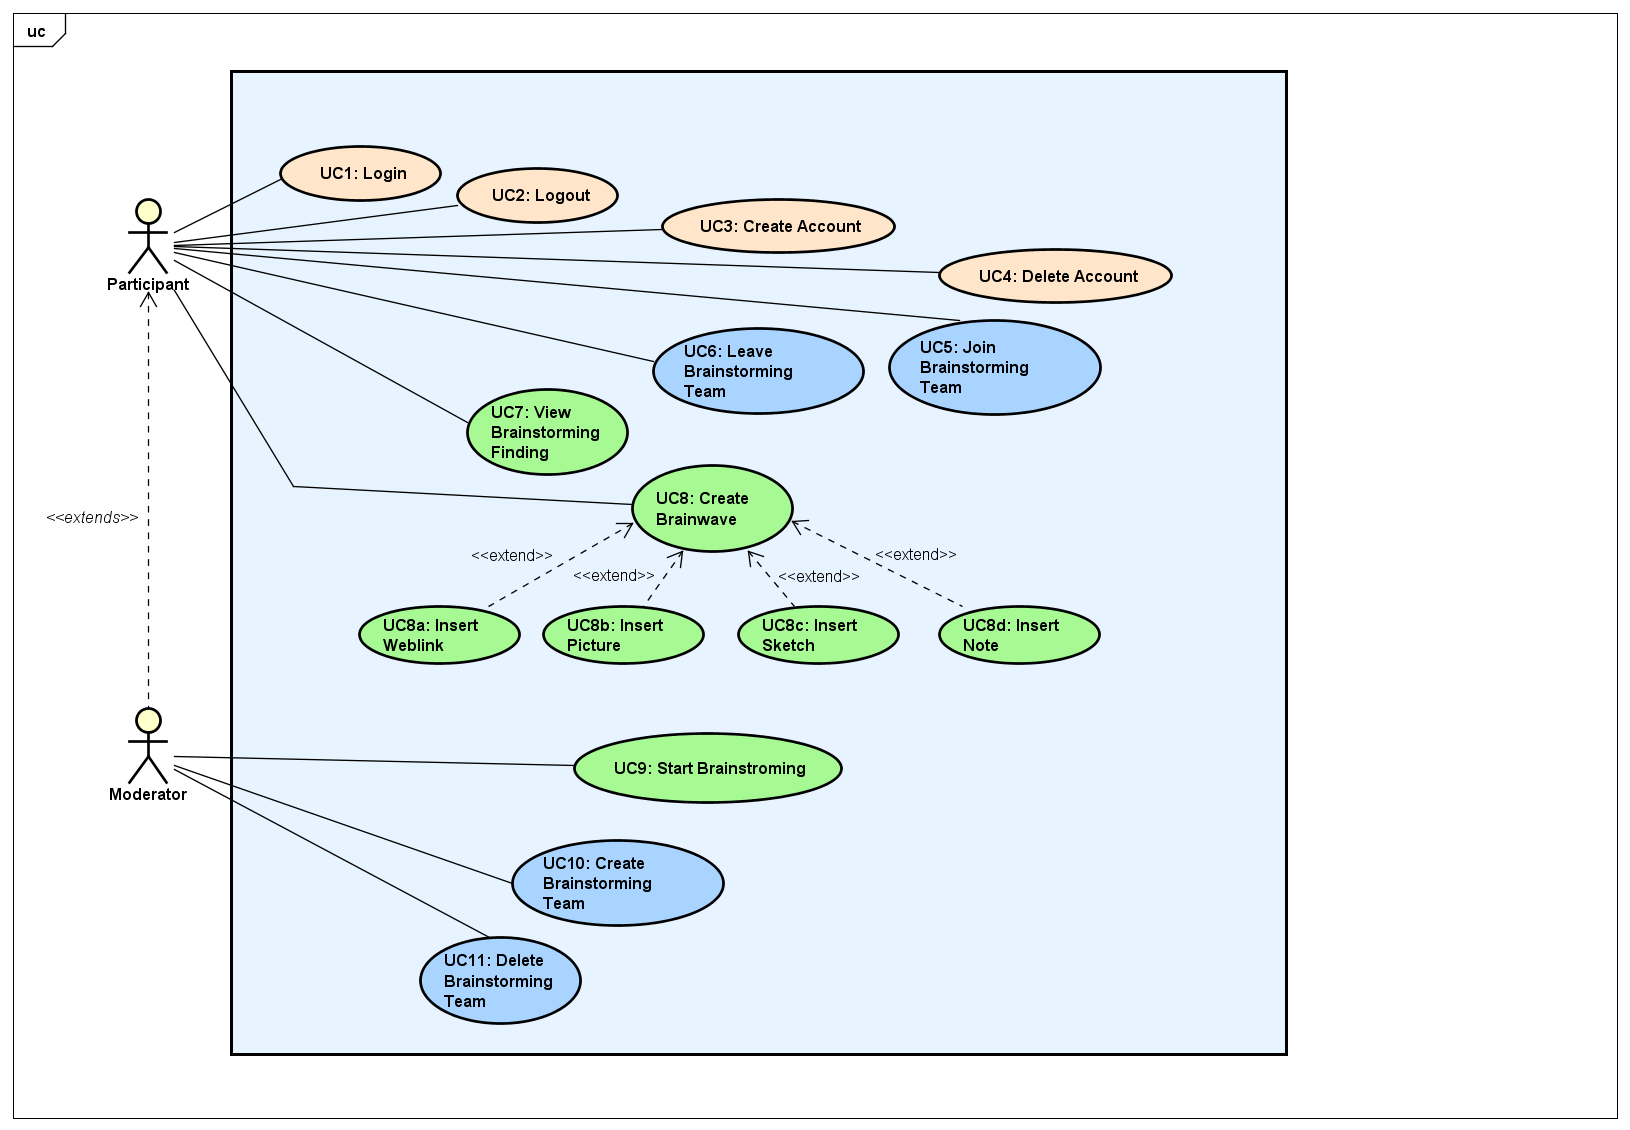
\includegraphics[width=1\linewidth]{./img/anforderungen/UC-Methode635.png}
	\caption{Use-Case Diagramm Methode 635}
	\label{fig:uc-methode635}
\end{figure}
Abbildung \ref{fig:uc-methode635} zeigt das Use-Case Diagramm für diese Arbeit. Es gibt einige Abweichungen zur Studienarbeit. Im Diagramm sind einige Use-Cases in blasser Farbe, bei diesen handelt es sich um bereits implementierte Features im Umfang der Studienarbeit. 

Wichtig zu erwähnen ist dabei, dass UC12: Create Brainstorming Finding erst im Nachhinein hinzugekommen ist. Dies ist so, weil zu Beginn der Entwicklung wir die Annahme trafen, dass für jedes Team genau ein Brainstorming entsteht und zwar zum Zeitpunkt des Starts des Brainstorming Findings (UC9). Wie wir aber im Verlaufe der Zeit feststellten, war die Umsetzung mit mehreren Brainstorming Findings pro Team keinen grossen Aufwand. So entstand ein zusätzlicher Use-Case, der nicht mehr implizit mit UC9: Start Brainstorming Finding ausgeführt wurde.

Weiter sind Use-Cases in satter Farbe erkennbar. Bei diesen handelt es sich um diejenigen, welche in dieser Arbeit im Fokus liegen. Komplett neu hinzugekommen sind UC8e: Insert Pattern und UC8f: Insert Video. Als zentralen Use-Case wird zudem UC8c: Insert Sketch angesehen. Im folgenden Kapitel werden nun die in dieser Arbeit relevanten Use-Cases kurz beschrieben. Im Kapitel \ref{par:fully-dressed-uc} sind alle zu implementierenden Sub-Use-Cases von UC8: Create Brainwave im fully-dressed Stil detailliert erläutert.
\paragraph{Brief Use-Cases}

\begin{basedescript}{
		\desclabelstyle{\multilinelabel}
		\desclabelwidth{4.5cm}
		\setlength{\itemsep}{5ex}}
	
	\item[\textit{UC2: }Logout] Als eingeloggter Participant will ich mich ausloggen, sodass das Startfenster wieder erscheint.
	
	\item[\textit{UC6: }Leave Brainstorming Team] Als Participant will ich ein beigetretenes Team verlassen können.
		
	\item[\textit{UC8: }Create Brainwave] Als Participant will ich während einer Brainstorming Session ein Brainwave (bestehend aus mehreren Ideen) erstellen und einreichen können. 
	
	\item[\textit{UC8a: }Insert Weblink] Als Participant will ich einen Weblink in mein aktuelles Sheet einfügen können.
	
	\item[\textit{UC8b: }Insert Picture] Als Participant will ich ein Bild in mein aktuelles Sheet einfügen können.
	
	\item[\textit{UC8c: }Insert Sketch] Als Participant will ich in mein aktuelles Sheet zeichnen können.
	
	\item[\textit{UC8e: }Insert Pattern] Als Participant will ich aus Vorlagen software-relevante Patterns in mein aktuelles Sheet einfügen können.
	
	\item[\textit{UC8f: }Insert Video] Als Participant will ich ein Video aufnehmen und in mein aktuelles Sheet einfügen können.
	
	\item[\textit{UC11: }Delete Brainstorming Team] Als Moderator will ich ein Brainstorming Team löschen können.
\end{basedescript}
\vspace{1cm}

\paragraph{Fully-Dressed Use-Cases}\label{par:fully-dressed-uc}


\paragraph{Abuse-Cases}
\paragraph{Sequenzdiagramm}

\subsubsection{Nicht-Funktionale Anforderungen}
Wie schon in unserer Studienarbeit halten wir uns auch hier wieder an die Standards ISO 9126\cite{ISO9126} bzw. dessen Nachfolger ISO 25010\cite{ISO9126_ISO25010}. Beide ISO-Normen sind sich sehr ähnlich und liefern eine gute Checkliste für jegliche Art von Systemanforderungen.

\begin{figure}[h]
	\centering
	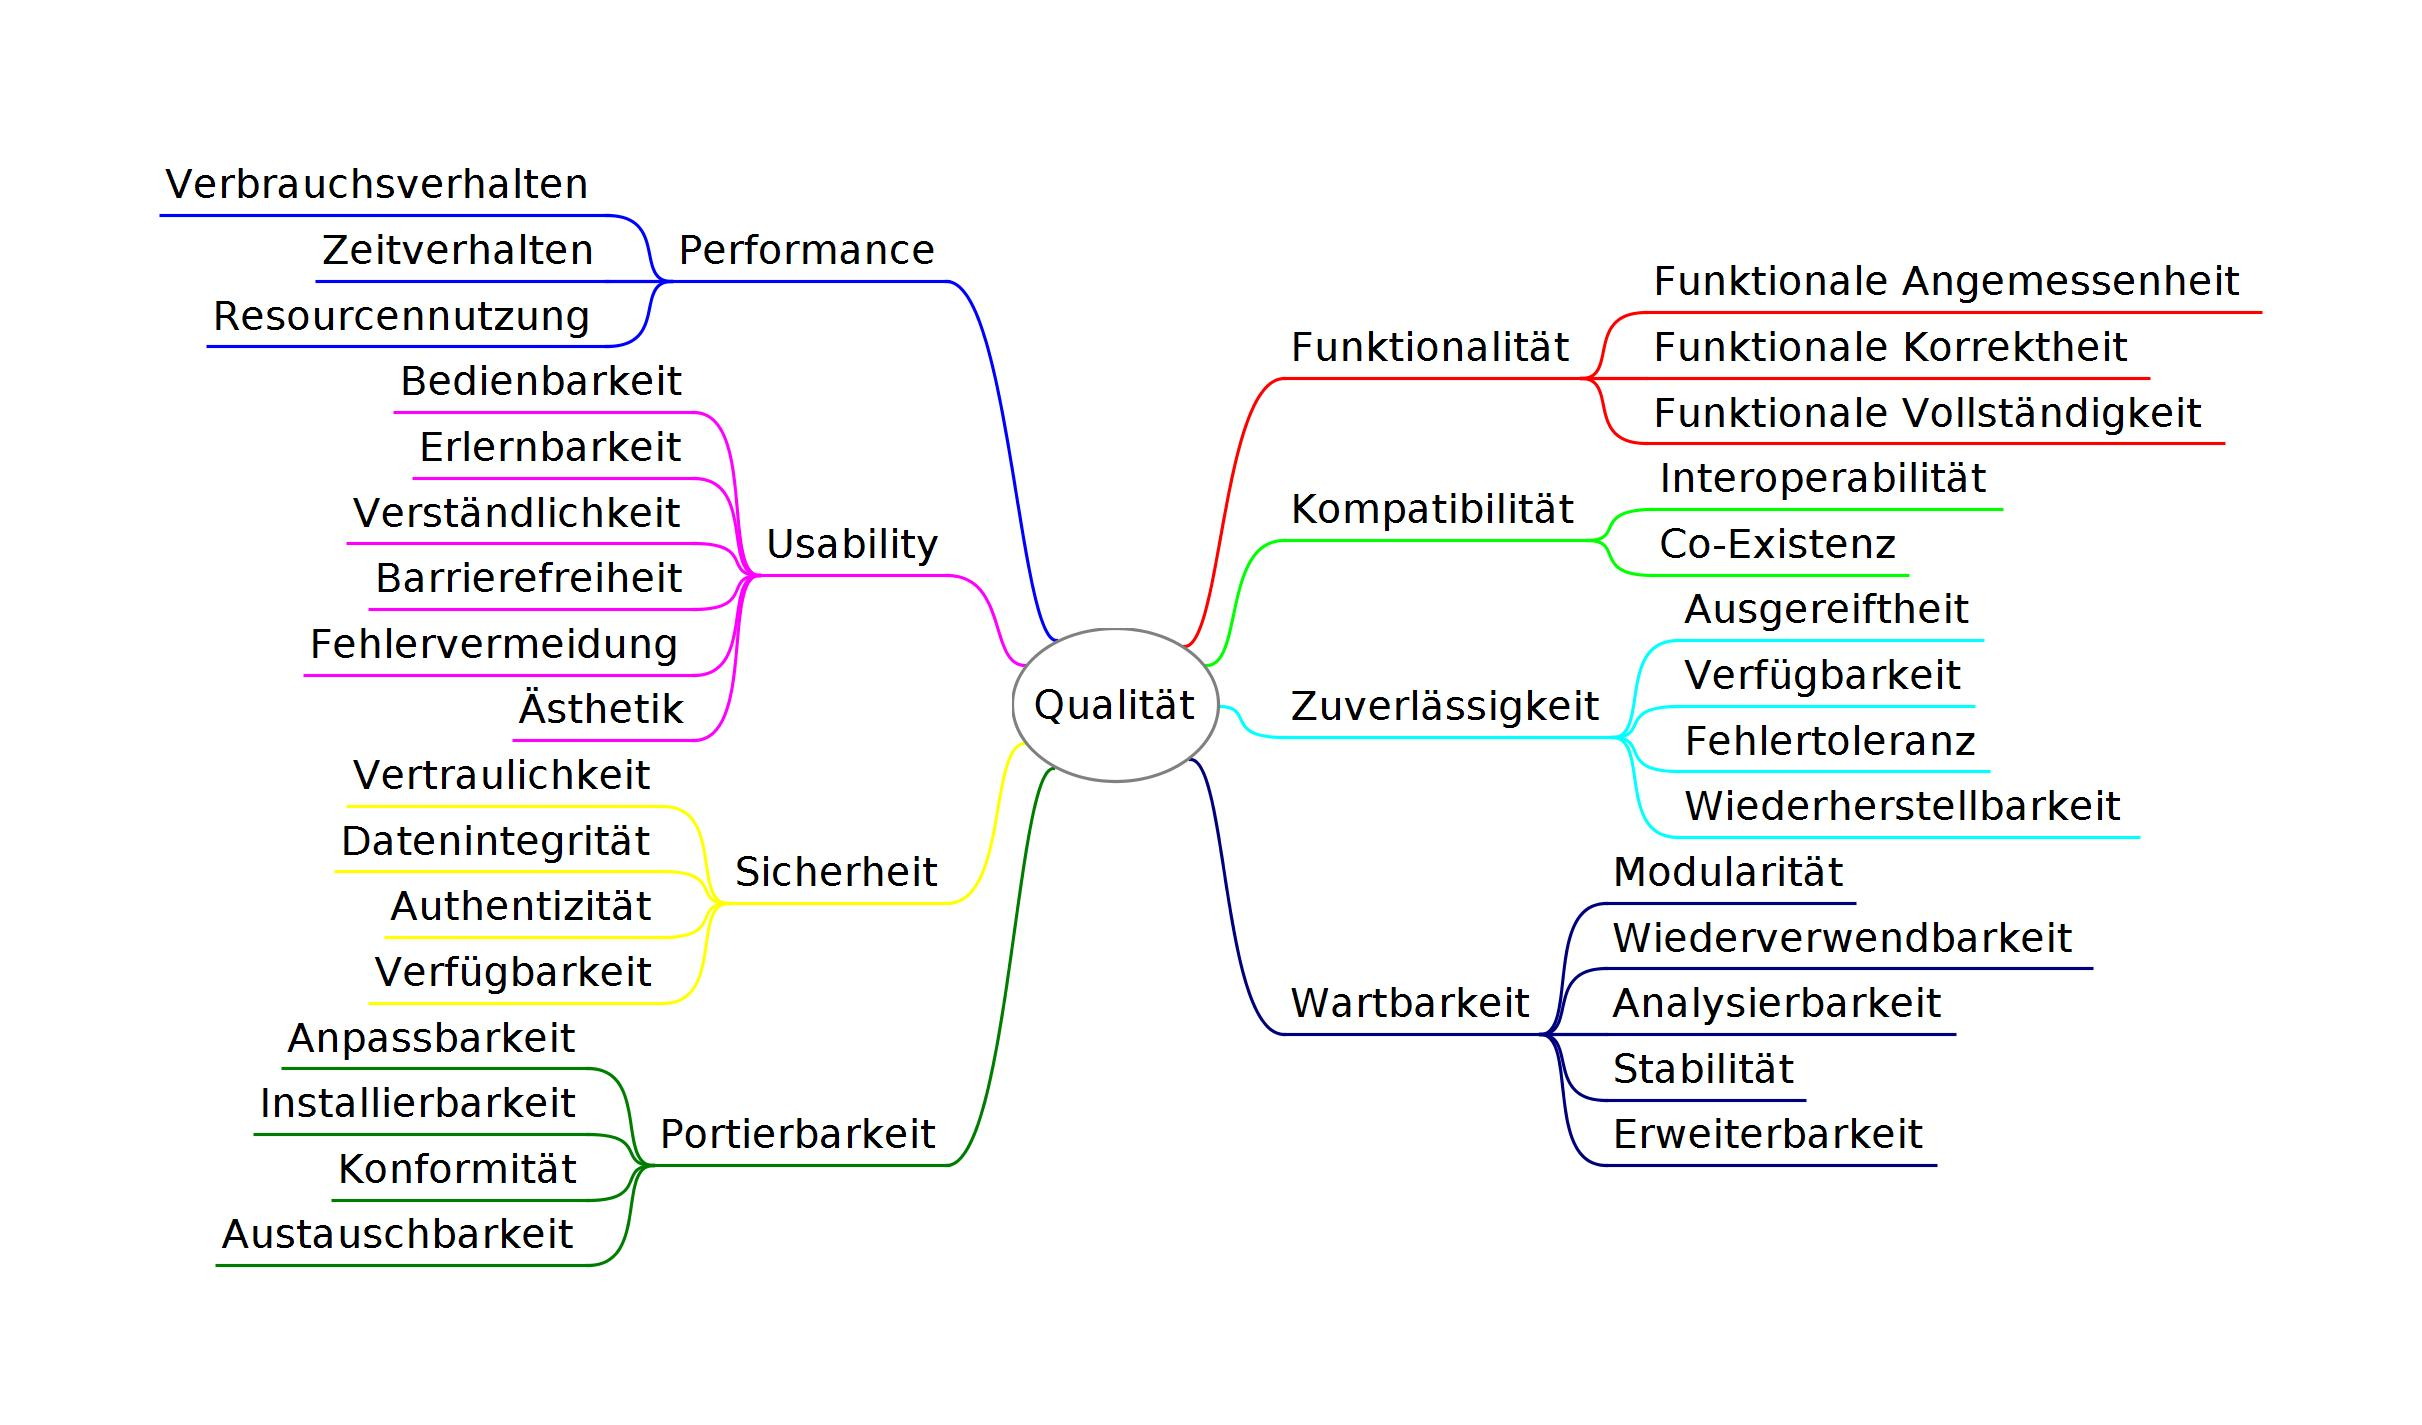
\includegraphics[width=1\linewidth]{img/anforderungen/quality}
	\caption[Anforderungskategorien nach ISO 25010]{Anforderungskategorien nach  ISO 25010}\cite{ISO25010_Bild}
	\label{fig:ISO 25010}
\end{figure}

Im Gegensatz zur Studienarbeit wollen wir uns bei dieser Arbeit aber vor allem auf Faktoren wie Erweiterbarkeit und Modularität konzentrieren. Auch sollen Faktoren wie Zeitverhalten und Ästhetik stärker in den Vordergrund rücken. 

Die bekannten nicht-funktionale Anforderungen aus der Studienarbeit bleiben allerdings weiter bestehen. Um genaue und erfüllbare nicht-funktionale Anforderungen zu definieren, müssen die SMART-Kriterien \cite{SMART} erfüllt sein.

\begin{center}
    \begin{tabular}{ | p{6cm} | p{2.5cm} | p{2.5cm} | p{2.5cm} |}
    	\hline
    Kriterium & Minimum & Optimal & Übertroffen \\ 
    	\hline
    \textbf{Zeitverhalten} \newline Zeitkritische Kommunikation (Abgabe von Ideen/Brainsheets) zwischen Server und App beträgt: & 2 Sekunden & 1 Sekunden & weniger als 1 Sekunde \\
    	\hline
    \textbf{Erweiterbarkeit} \newline Die Anzahl an neuen Modularten (Problem-Arten), welche mit der bestehenden Architektur als umsetzbar gelten, wird als ... angesehen: & zu wenig & ausreichend & unbegrenzt \\
    	\hline
    \textbf{Modularität} \newline Die App ist innert ... Tagen um ein neues Modul (Problem-Art) erweitert: & 5 Tage & 2 Tage & weniger als 1 Tag \\
    	\hline
    \textbf{Ästhetik} \newline Die Anziehungskraft gegenüber dem Endnutzer wird als ... charakterisiert: & gering & in Ordnung & süchtig \\
    	\hline
    \textbf{Ausgereiftheit} \newline Der Grad der Ausgereiftheit oder Reife wird als ... angesehen: & ungenügend für den produktiven Einsatz (Prototypen-Stadium) & genügend für den produktiven Einsatz, kann aber immer noch in Fehlerzustände gelangen & kaum Fehlerzustände und somit keine Abstürze der App  \\
    	\hline
    \end{tabular}
\end{center}

\newpage

\subsection{Domainanalyse}

Das Domain-Modell besteht grob aus zwei Teilen: den Benutzern und der Brainstorming Methodik. 

Dabei bilden mehrere Participants ein \textit{Brainstorming Team}. Diese wird von einem der Participants, dem \textit{Moderator}, gegründet.  Das Team hat die Möglichkeit, ein oder mehrere \textit{Brainstorming Findings} zu erarbeiten. Dies entspricht einer gesamten Durchgang der Methode. Der Moderator erstellt diese und hat die Möglichkeit, die Anzahl von Ideen sowie die erste Rundenzeit zu konfigurieren. Jede weitere Runde wird um eine Minute verlängert.

Das \textit{Brainsheet} entspricht einem physikalischem Blatt, das herumgegeben wird. In der Standardkonfiguration 635 existieren also 6 Sheets (weil 6 Teilnehmer dabei sind).

Eine \textit{Brainwave} ist das Produkt jedes Participants am Ende einer Runde. Es gehört in ein Brainsheet, das jede Runde an den nächsten Participant weitergegeben wird. In der Standardkonfiguration besteht eine Brainwave aus 3 Ideen (6\textbf{3}5).

Die \textit{Idea} ist ein effektiv erarbeiteter Teil einer Brainwave. Im Normalfall ist eine Idee simpler Text (\textit{NoteIdea}), wobei weitere Typen von Ideen (Bild, Weblink und Zeichnung) durch das verwendete Design erdenklich sind. Speziell erwähnenswert ist der Umstand, dass im Gegensatz zur Studienarbeit, neu die Ideentypen VideoIdea und PatternIdea angedacht sind.

\begin{figure}[h]
	\centering
	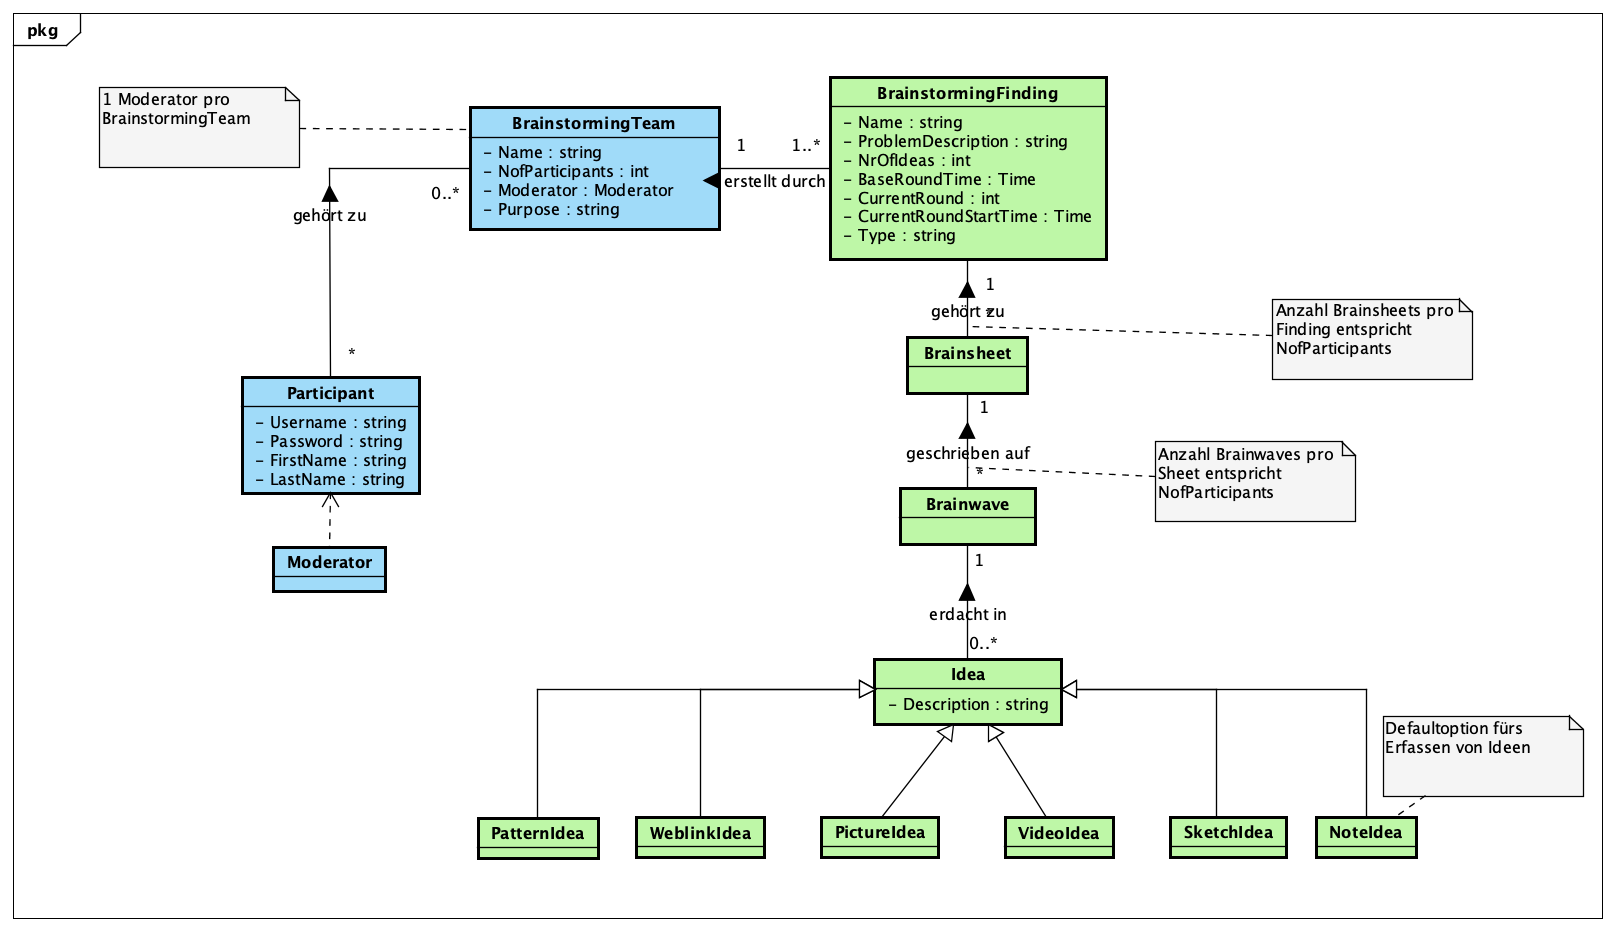
\includegraphics[width=1\linewidth]{img/domain-analyse/DomainModell-Methode635}
	\caption{Domain Modell BrainingOutOfBox}
	\label{fig:domainmodell-methode635}
\end{figure}


\newpage

\subsection{Architekturdokumentation}
\label{architektur}
In diesem Kapitel gehen wir detailliert in die Architektur und das Deployment unseres Projektes ein.

\subsubsection{Logische Architektur}

\paragraph*{Komponenten}
\subsubsection{Deployment}
\paragraph*{Komponenten}

\newpage

\subsection{Architekturentscheide}
Wesentliche Entscheide, welche wir während dem Projekt getroffen haben, sind hier detailliert begründet. Auch Gedanken oder Ideen, welche wir während der Analysephase hatten, dann aber verworfen haben, sind hier aufgeschrieben.

\newpage

\subsection{Herausforderungen}
Hier sind besonders erwähnenswerte Herausforderungen und Hürden beschrieben, die im Verlaufe des Projektes aufkamen. Dies soll anderen Software Ingenieuren oder Interessierten helfen, aus unseren Schwierigkeiten zu lernen. 


\subsubsection{Navigationsprobleme mit Prism Forms}\label{subsub:navigation}

Die grösste Herausforderung im Frontend war die Navigation mit Prism Forms und Xamarin Forms. Ein zentraler Unterschied liegt in der absolution und relativen Navigation. Bei der absoluten Navigation wird der gesamte Navigationsstack bei jedem Aufruf neu aufgebaut, was zur Folge hat, dass alle beteiligten ViewModels neu erstellt (Konstruktoraufruf) werden und darauf navigiert wird (Aufruf von \texttt{OnNavigatedTo} und \texttt{OnNavigatedFrom}). Dies im Unterschied zur relativen Navigation, wo jeweils die zu navigierende Page auf den Stack gelegt wird und nur die Methoden auf dem zuständigen ViewModel aufgerufen werden. 

Das Problem war nun, dass wir uns im Kontext einer \texttt{TabbedPage} bewegen und die Navigationsschritte bei einem Klick auf einem Element in einem Tab auf ein anderes Tab wechseln müssen. Leider funktioniert in diesem Zusammenhang nur die absolute Navigation, weil wir innerhalb einer Page mit den verschiedenen Tabs navigieren wollen und die Navigation von Prism Forms dazu implementiert wurde, zwischen Pages zu navigieren. Dies hat zur Folge, dass jeder Tabwechsel mit absoluter Navigation entwickelt werden musste. Der gesamte Code muss also berücksichtigen, dass die ViewModels mehrmals initialisiert werden und somit Instanzen überschrieben und verändert werden können. Dies ist ein erheblicher Mehraufwand, der immer wieder zu Fehlverhalten und viel zusätzlichem Code führte. 

Im späteren Projektverlauf wurde festgestellt, dass der Navigationservice von Prism Forms um eine Methode namens \texttt{SelectTab()} erweitert wurde \cite{prism-selecttab}, was die beschriebene Problematik lösen könnte. Jedoch ist diese Extensionmethode noch nicht im stabilen Release von Prism Forms und daher noch nicht nutzbar. In einer Folgearbeit ist es sehr empfehlenswert, diese Funktionalität zu testen und zu verwenden. 


\newpage

\subsection{Ergebnisse}
Das Kapitel der Ergebnisse befasst sich mit der konkreten Umsetzung der gesamten Applikation und dokumentiert die grundlegenden Ergebnisse oder Resultate, welche aus dieser Arbeit hervorgegangen sind. 

Auch hier soll nochmals erwähnt sein, dass diese Arbeit auf der Studienarbeit \cite{methode635-sa} aufbaut und grundlegende Informationen dort nachzulesen sind. 

In diesem Kapitel gehen wir zunächst auf die Änderungen während der Refactoring-Phase ein und schildern was dies für die Wartung und Erweiterung des Codes bedeutet. 

Anschliessend sind weitere Features dokumentiert, welche im Verlauf dieser Arbeit an der Applikation durchgeführt wurden.

Das Kapitel wird durch eine Gegenüberstellung der erreichten und geplanten Arbeit abgeschlossen.

Zur besseren Übersicht wurde der Code vereinzelt gekürzt. Dies ist durch 3 Punkte (...) gekennzeichnet.

\subsubsection{Refactoring zu Beginn der Arbeit}
Wie aus dem Projektplan (siehe Abbildung \ref{fig:projekt-plan}) zu entnehmen ist, haben wir uns zu Beginn unserer Arbeit dazu entschieden, zwei Sprints für das Refactoring unsere Applikation zu nutzen. Die Entscheidung überhaupt ein Refactoring durchzuführen entstand aus der Tatsache, dass wir schon gegen Ende der Studienarbeit gemerkt hatten, dass bei einer allfälligen Weiterführung der Arbeit ein Refactoring von grossem Wert sein wird. Auch haben wir diesbezüglich schon während der Studienarbeit einzelne Vorschläge für ein Refactoring beschrieben.


Das Ziel der Refactoring-Phase war es daher, den Code, welcher aus der Studienarbeit hervorgegangen ist, zu prüfen und zu verbessern. Dies sollte uns helfen, die Erweiterbarkeit für zukünftig geplante Features zu gewähren.

Auch konnten wir die in der Studienarbeit beschriebenen Vorschläge erfolgreich in der App umsetzen.
 
\paragraph*{Refactoring Backend}~\\
Dieser Abschnitt ist so aufgebaut, dass anhand von zwei Beispielen aufgezeigt werden soll, wie der Code im Backend vor und nach dem Refactoring ausgesehen hat. Auch wird am Ende des Abschnitts kurz erwähnt, was dies für Verbesserungen zur Folge hatte.

Das nachfolgende Listing \ref{participantErstellenVorRef} zeigt einen Ausschnitt aus der \texttt{Participant\-Controller} Klasse wie es vor dem Refactoring war. Das Listing \ref{participantErstellenNachRef} zeigt dieselbe Methode nach dem Refactoring.

\lstset{language=JAVA, showstringspaces=false, frame=single, captionpos=b, label=createParticipant, breaklines=true, numbers=left}
\begin{lstlisting}[caption={Participant erstellen vor Refactoring}, label=participantErstellenVorRef]
public Result createParticipant(){

    JsonNode body = request().body().asJson();

    if (body == null ) {
        return forbidden(Json.toJson(new ErrorMessage("Error", "json body is null")));
    } else if(  body.hasNonNull("username") &&
            	body.hasNonNull("password") &&
            	body.hasNonNull("firstname") &&
            	body.hasNonNull("lastname")) {

    Participant participant = new Participant(body.get("username").asText(), body.get("password").asText(), body.get("firstname").asText(), body.get("lastname").asText());

    participantCollection.insertOne(participant, new SingleResultCallback<Void>() {
        @Override
        public void onResult(Void result, Throwable t) {
            Logger.info("Inserted Participant!");
        }
    });

    return ok(Json.toJson(new SuccessMessage("Success", "Participant successfully inserted")));
    }

    return forbidden(Json.toJson(new ErrorMessage("Error", "json body not as expected")));
}
\end{lstlisting}

\begin{lstlisting}[caption={Participant erstellen nach Refactoring}, label=participantErstellenNachRef]
@BodyParser.Of(ParticipantDTOBodyParser.class)
public Result createParticipant() {
    ParticipantDTO participantDTO = request().body().as(ParticipantDTO.class);
    Participant participant = modelsMapper.toParticipant(participantDTO);

    try {
        if (service.insertParticipant(participant)){
            return ok(Json.toJson(new SuccessMessage("Success", "Participant successfully inserted")));
        } else {
            Logger.info("Username already exists");
            return badRequest(Json.toJson(new ErrorMessage("Error", "Username already exists")));
        }
    } catch (ExecutionException | InterruptedException e) {
        return internalServerError(Json.toJson(new ErrorMessage("Error", e.getMessage())));
    }
}
\end{lstlisting}

Das Erstellen des Participants wurde komplett in den \texttt{Participant\-DTO\-Body\-Parser} ausgelagert. Dieser erstellt nun aus dem angelieferten JSON (JavaScript Object Notation) ein Data-Transfer-Object \cite{DTO}, welches in einem nächsten Schritt zu einem Business Object aufgelöst wird (Zeile 4).

Jegliche Überprüfungen aus Listing \ref{participantErstellenVorRef} (Zeilen 5 und 7-10) konnten so zentral in den BodyParser ausgelagert werden.

Bei den nachfolgenden Listings \ref{putBrainsheetVorRef} und \ref{putBrainsheetNachRef}, welche einen Ausschnitt aus dem \texttt{Brain\-storming\-Finding\-Controller} zeigen, ist der Unterschied noch stärker zu sehen. So konnte zum Beispiel die \texttt{putBraisheet} Methode von zirka 40 Zeilen auf 15 Zeilen gekürzt werden. 

\begin{lstlisting}[caption={PutBrainsheet vor Refactoring}, label=putBrainsheetVorRef]
public Result putBrainsheet(String findingIdentifier) throws ExecutionException, InterruptedException {

JsonNode body = request().body().asJson();
JsonNode brainwaves = body.findPath("brainwaves");
JsonNode nrOfSheet = body.findPath("nrOfSheet");

if (body == null ) {
    return forbidden(Json.toJson(new ErrorMessage("Error", "json body is null")));
} else if(  !brainwaves.isNull() &&
            !nrOfSheet.isNull()){

	BrainstormingFinding finding = getBrainstormingFinding(findingIdentifier);

    if (finding == null){
        return internalServerError(Json.toJson(new ErrorMessage("Error", "No brainstormingFinding found")));
    }

    Brainsheet oldBrainsheet = finding.getBrainsheets().get(nrOfSheet.asInt());
    Brainsheet newBrainsheet = createBrainsheet(body);


    findingCollection.updateOne(eq("identifier", findingIdentifier),pullByFilter(Filters.eq("brainsheets", oldBrainsheet)), new SingleResultCallback<UpdateResult>() {
        @Override
        public void onResult(final UpdateResult result, final Throwable t) {
            Logger.info(result.getModifiedCount() + " Brainsheet successfully deleted");
        }
    });

    findingCollection.updateOne(eq("identifier", findingIdentifier),combine(pushEach("brainsheets", Arrays.asList(newBrainsheet), new PushOptions().position(newBrainsheet.getNrOfSheet())), inc("deliveredBrainsheetsInCurrentRound", 1)), new SingleResultCallback<UpdateResult>() {
        @Override
        public void onResult(final UpdateResult result, final Throwable t) {
            Logger.info(result.getModifiedCount() + " Brainsheet successfully inserted");
        }
    });

    return ok(Json.toJson(new SuccessMessage("Success", "Brainsheet successfully updated")));
}

return forbidden(Json.toJson(new ErrorMessage("Error", "json body not as expected")));
}
\end{lstlisting}


\begin{lstlisting}[caption={PutBrainsheet nach Refactoring}, label=putBrainsheetNachRef]
@BodyParser.Of(BrainsheetDTOBodyParser.class)
public Result putBrainsheet(String findingIdentifier){
    BrainsheetDTO brainsheetDTO = request().body().as(BrainsheetDTO.class);
    Brainsheet newBrainsheet = modelsMapper.toBrainsheet(brainsheetDTO);

    try {

        if (service.exchangeBrainsheet(findingIdentifier, newBrainsheet)) {
            return ok(Json.toJson(new SuccessMessage("Success", "Brainsheet successfully updated")));
        } else {
            return badRequest(Json.toJson(new ErrorMessage("Error", "No Brainsheet updated")));
        }

    } catch (ExecutionException | InterruptedException e) {
        return internalServerError(Json.toJson(new ErrorMessage("Error", e.getMessage())));
    }
}
\end{lstlisting}

Die gesamte Logik für den Austausch der Brainsheets wurde in die \texttt{FindingService} Klasse ausgelagert.

\begin{lstlisting}[caption={Exchange Brainsheet im Business Layer}, label=exchangeBrainsheetBusinessLayer]
public boolean exchangeBrainsheet(String findingIdentifier, Brainsheet newBrainsheet) {
BrainstormingFinding finding = service.getFinding(findingIdentifier).get();
if (finding == null){
    return false;
} else {
    if (newBrainsheet.getNrOfSheet() < finding.getBrainsheets().size()) {
       service.exchangeBrainsheet(finding, newBrainsheet);
       return true;
    }
    return false;
}
}
\end{lstlisting}

Auch wurde die Implementation für das Einfügen in die Datenbank in eine separate Klasse (\texttt{MongoDBFindingService}) ausgelagert, um eine bessere Übersicht und ein besseres Layering zu gewähren.

\begin{lstlisting}[caption={Exchange Brainsheet im Data Access Layer}, label=exchangeBrainsheetDAL]
public void exchangeBrainsheet(BrainstormingFinding finding, Brainsheet newBrainsheet){
    
//update Brainsheet at the correct index
findingCollection.updateOne(eq("identifier", finding.getIdentifier()),combine(set("brainsheets."+newBrainsheet.getNrOfSheet(), newBrainsheet), inc("deliveredBrainsheetsInCurrentRound", 1)), (result, t) -> Logger.info(result.getModifiedCount() + " new Brainsheet successfully updated"));
}
\end{lstlisting}
Diese zwei Beispiele stellen noch lange nicht alle überarbeiteten Codestellen dar, geben aber eine gute Übersicht, wie der gesamte Code vereinfacht werden konnte.

\paragraph*{Fazit}~\\
Gerade das Beispiel vom Austausch der Brainsheets (Listing \ref{putBrainsheetVorRef}) verdeutlicht, dass das Layering stark verbessert wurde. Damit konnte die Übersicht und Komplexität deutlich verbessert werden.

Auch wurden im gesamten Backend Data-Transfer-Obekte (DTO) \cite{DTO} eingefügt. Die Idee von DTOs ist es, alle Daten, welche über das Netzwerk gesendet werden in eben jenen Data-Transfer-Obekten zu speichern und zu übertragen. Im Unterschied zu den Business-Objects besitzen DTOs kein business-relevantes Verhalten. Sie sind ausschliesslich für die Übertragung der Daten verantwortlich. Dies war vor allem im späteren Verlauf der Arbeit von grossem Wert.

Mit Hilfe der BodyParser-Klassen konnte die komplette Überprüfung und Deserialisierung der angelieferten JSON-Daten zentral geregelt werden. Somit ist immer sichergestellt, dass das DTO korrekt (alle erwarteten Informationen sind vorhanden und das Format stimmt) erstellt wird. 

\paragraph*{Refactoring Frontend}~\\
Auf der Seite des Frontends standen folgende Punkte für das Refactoring an:
\begin{enumerate}
	\item Performanceverbesserung
	\item State Machine für die Brainstorming Logik
	\item Services, allgemeines Layering
	\item Einfügen von DTOs
	\item Logger
	\item Localisation
\end{enumerate}

Zuerst wurde ein einfaches Layering vorgenommen. Alle Models wurden in ein separates Projekt ausgelagert und verwendet. Zusätzlich wurden einzelne Services wie der \texttt{UiNavigationService} erstellt, welcher jegliche Navigationsschritte ausführen kann und in die ViewModels injected wird. Durch das Einführen dieses Services hat sich bereits ein grösseres Problem gelöst: die Performance Issues. Vor diesem Service rief jedes ViewModel den durch das MVVM-Framework PrismForms bereitgestellten \texttt{NavigationService} auf. Dies führte dazu, dass bei jedem Navigationsschritt der \texttt{NavigationService} neu initialisiert wurde. Durch das Kapseln in eine eigene Klasse kann dieser als Singleton im IoC Container registriert werden, somit wird dieser nur beim Starten der Applikation initialisiert. 

Nachdem die Navigation in einen Service ausgelagert wurde, musste die Implementation der Kern-Logik überarbeitet werden. Dazu wurde im Umfang der Studienarbeit bereits ein Konzept für eine State-Machine erarbeitet \cite{methode635-sa}. Diese wurde mittels Test-Driven-Design in der jetzigen Arbeit umgesetzt. Listing \ref{start-statemachine} zeigt, wie die Statemachine beim Start ermittelt, in welchem State sie sich befindet.
\begin{lstlisting}[caption=Start der Klasse StateMachine, label=start-statemachine]
public void Start()
{
	var currentRound = _context.CurrentFinding.CurrentRound;
	IState evaluatedState = null;
	if (currentRound == -1)
	{
		evaluatedState = new EndedState(_context, _brainstormingModel);
	}
	else if (currentRound == 0)
	{
		evaluatedState = new WaitingState(_logger, _brainstormingDalService, _context, _brainstormingModel);
	}
	else if (currentRound > 0)
	{
		evaluatedState = new RunningState(_logger, _brainstormingDalService, _context, _brainstormingModel);
	}
	if(currentRound < -1 || evaluatedState == null)
	{
		throw new ArgumentException("Invalid round or state not registered");
	}
	ChangeState(evaluatedState);
}
\end{lstlisting}
Wie auf Zeile 4 ersichtlich wurde gegen ein Interface namens \texttt{IState} programmiert. Dieses Interface enthält eine \texttt{Init()}- und eine \texttt{CleanUp()}-Methode, sowie ein \texttt{PropertyChanged}-Event, der für das Notifizieren der Änderungen eines States zuständig ist. Durch das \texttt{IState}-Interface ist die Erweiterbarkeit gewährleistet (z.B. Einführen eines zusätzlichen 'Review' States). 

Die StateMachine musste anschliessend von einem Service verwendet werden. Der \texttt{BrainstormingService} ist für die gesamte Kernlogik zuständig und behält somit eine Instanz der \texttt{StateMachine}. Auch im \texttt{BrainstormingService} wurde gegen ein Interface programmiert. Dessen Methoden sind der Abbildung \ref{fig:ibrainstormingservice} zu entnehmen.

\begin{figure}[h]
	\centering
	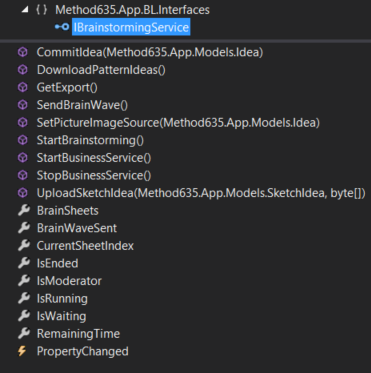
\includegraphics[width=0.5\linewidth]{img/techn-bericht/ibrainstormingservice}
	\caption{Methoden des IBrainstorming-Interfaces}
	\label{fig:ibrainstormingservice}
\end{figure}

Neben diesen erwähnten Services wurden auch Services im Data-Access-Layer (DAL) eingeführt. Diese sind in einem separaten Projekt und können ebenfalls mittels deren Interface in die verwendenden Klassen injiziert werden. Sie sind für den gesamten Daten-Zugriff zuständig. Für das Abbilden der Endpunkte des Backends, wurde weiter ein Konfigurationsfile eingeführt. Dieses Json-File wird geparst und vom \texttt{ConfigurationService} den Repositories zur Verfügung gestellt. 

Für das Einführen von DTOs wurde wie zu Beginn dieses Kapitels erwähnt, dass alle Models in ein separates Projekt ausgelagert wurde. Im DAL existiert ein Ordner mit DTOs, welche für das Parsen der Objekte vom Backend verwendet werden. Es wurde zusätzlich ein Mapping-Layer eingeführt, der die Objekte in die Business Objekte abbildet. Dazu wurde das NuGet-Packet Automapper verwendet. 

Das Auslagern und Zerstückeln der Logik in Services und das Verwenden von Interfaces erleichterte uns die Implementation der nachfolgend beschriebenen Features erheblich. Weiter konnten besonders durch die verschiedenen States in der \texttt{StateMachine} späteres Fehlverhalten viel besser eingeschränkt und korrigiert werden. 

\subsubsection{Implementation Skizzen Feature}
Die Skizzen-Funktion soll es dem Endnutzer ermöglichen, nebst den \texttt{NoteIdeas} auch \texttt{SketchIdeas} (siehe Abbildung \ref{fig:domainmodell-methode635}) zu erfassen. Mit den \texttt{SketchIdeas} wird dem Endnutzer die Möglichkeit gegeben, Skizzen als Teil der Brainstorming-Runden zu zeichnen.

Da es sich bei den einzelnen Skizzen um Binärdaten handelt, musste zunächst eine Möglichkeit geschaffen werden, diese Art von Daten in der Datenbank abzulegen. Dafür wurden in der Elaboration-Phase Analysen (siehe Kapitel \ref{seq:save_file_in_db}) durchgeführt und ein Prototyp erstellt, um die technische Machbarkeit zu verifizieren.

\paragraph*{Implementation Backend}~\\
In den nachfolgenden Listings wird aufgezeigt, wie die Sketch-Funktion im Backend umgesetzt wurde.
Der genaue Kommunikations-Ablauf kann der Abbildung \ref{fig:Seq-Draw-Sketch} in Kapitel \ref{par:sequence-diagramm} entnommen werden.

\begin{lstlisting}[caption={Upload File im File Controller}, label=uploadFileController]
@BodyParser.Of(MultipartFormDataBodyParser.class)
public Result uploadFile(){
    try {

    final Http.MultipartFormData<File> formData = request().body().asMultipartFormData();
    final Http.MultipartFormData.FilePart<File> filePart = formData.getFile("name");
    final File file = filePart.getFile();

    final byte[] fileData = Files.readAllBytes(file.toPath());
    final String fileName = file.getName();

    String fileId = service.uploadFileAsStream(fileData, fileName);
    return ok(Json.toJson(new SuccessMessage("Success", fileId)));

    } catch (IOException | InterruptedException | ExecutionException  e) {
        return internalServerError(Json.toJson(new ErrorMessage("Error", e.getMessage())));
    }
}
\end{lstlisting}

Ähnlich wie bei den JSON-Daten, wird auch hier zunächst die Skizze mittels eines BodyParsers (Zeile 1) in ein File (in-Memory) umgewandelt (Zeilen 5-7), welches dann als Byte-Array dem File-Service (Zeile 12) übergeben werden kann. 

\begin{lstlisting}[caption={Upload File im File Service}, label=uploadFileService]
public String uploadFileAsStream(byte[] stream, String fileName) ... {
    return service.uploadFileAsStream(stream,fileName);
}
\end{lstlisting}

Der File-Service nimmt das Byte-Array entgegen und gibt dieses unverändert dem Datenbank-Service weiter.

\begin{lstlisting}[caption={Upload File im DB Service}, label=uploadFileDBService]
@Override
public String uploadFileAsStream(byte[] stream, String fileName) ... {
    ByteBuffer data = ByteBuffer.wrap(stream);
    CompletableFuture<String> future = new CompletableFuture<>();

    final GridFSUploadStream uploadStream = gridFSBucket.openUploadStream(fileName);
    uploadStream.write(data, (result, t) -> {
        Logger.info("File successfully inserted; ID: " + uploadStream.getObjectId().toHexString());
        future.complete(uploadStream.getObjectId().toHexString());

        uploadStream.close((result1, t1) -> {
            // stream close
        });
    });

    return future.get();
}
\end{lstlisting}

Der Datenbank-Service speichert anschliessend das Bild in die Datenbank (Zeile 7) und liefert bei erfolgreicher Speicherung die ObjektID zurück (Zeile 9). Am Ende wird noch der uploadStream zur Datenbank geschlossen (Zeile 11).

Die Smartphone-Applikation speichert nun die ObjektID als Teil der \texttt{SketchIdea} und sendet das \texttt{Brainsheet} wie gewohnt nach Ablauf der Zeit an das Backend.

Das Herunterladen der gespeicherten Bilder funktioniert auf ganz ähnliche Weise. Da die ObjektID in der \texttt{SketchIdea} abgelegt ist, kann das eigentliche Bild problemlos wiedergefunden werden.

\begin{lstlisting}[caption={Download File im DB Service}, label=uploadFileDBService]
@Override
public byte[] downloadFileAsStream(String id) ...{
    ObjectId fileId = new ObjectId(id);
    final ByteBuffer dstByteBuffer = ByteBuffer.allocate(1024 * 1024);
    final GridFSDownloadStream downloadStream = gridFSBucket.openDownloadStream(fileId);
    CompletableFuture<byte[]> future = new CompletableFuture<>();

    downloadStream.read(dstByteBuffer, (result, t) -> {
        dstByteBuffer.flip();
        byte[] bytes = new byte[result];
        dstByteBuffer.get(bytes);
        Logger.info("Found file to download; Size: " + result);
        future.complete(bytes);

        downloadStream.close((result1, t1) -> {
            // stream closed
        });
    });
    return future.get();
}
\end{lstlisting}

Hierbei wird ein downloadStream geöffnet, welcher die Daten anhand der ID aus der Datenbank liest und in ein Byte-Array schreibt (Zeile 8). Auch hier wird am Ende der Stream wieder geschlossen (Zeile 15).

Der zurückgelieferte Byte-Array wird anschliessend unverändert an den Client zurück\-geschickt. Allfällige Fehler während der Ausführung sowohl beim Hochladen wie auch beim Herunterladen werden im File-Controller abgefangen und als Fehler an den Client geschickt.

\paragraph*{Implementation Frontend}~\\
Das Feature wird im Frontend durch folgende Schritte während dem Brainstorming erreicht:
\begin{enumerate}
	\item Klicken des 'More Ideas'-Buttons, der auf zusätzliche Ideentypen hindeutet
	\item Auswählen des 'Sketch Idea' in der nächsten Ansicht
\end{enumerate}
Nachdem die Sketch-Ansicht erscheint, hat man Optionen zur Auswahl von Stiftgrösse und -farbe und kann die Skizze speichern oder die Zeichenfläche löschen.

Abbildung \ref{fig:sketch-page} verdeutlicht den Navigationsablauf.

\begin{figure}[h]
	\centering
	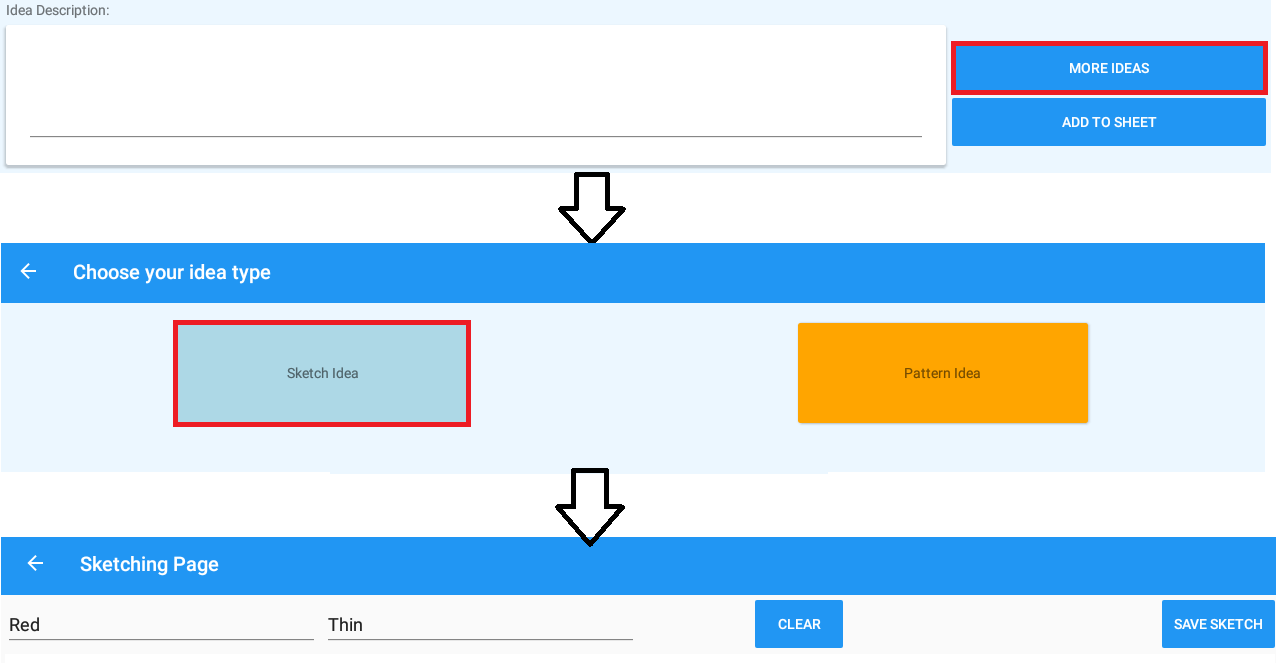
\includegraphics[width=1\linewidth]{img/techn-bericht/sketch-page}
	\caption{Navigationsablauf zur SketchPage}
	\label{fig:sketch-page}
\end{figure}

Durch das Betätigen des 'More Ideas'-Buttons wird der \texttt{UiNavigationService} aufgerufen, welcher wiederum auf die \texttt{InsertSpecialPage} navigiert. Dasselbe geschieht bei der Auswahl der 'Sketch Idea'-Kachel, nur wird dieses Mal die  \texttt{SketchPage} aufgerufen. 

Die Implementation der Sketching-Page hält sich stark an die Dokumentation von Microsoft \cite{sketching-xf}. Hinzu kam die Funktionalität, das Bild zu speichern und an das Backend zu schicken. Dazu muss ein Snapshot des Canvas' zum Zeitpunkt des Betätigen des 'Save-Image'-Buttons gemacht werden. Der Code dazu ist in Listing \ref{save-clicked-sketch} zu finden.

\begin{lstlisting}[label={save-clicked-sketch},caption={Save Click-Eventhandler}]
private void Save_Clicked(object sender, EventArgs e)
{
	var info = new SKImageInfo((int)canvasView.CanvasSize.Width, (int)canvasView.CanvasSize.Height);
	var surface = SKSurface.Create(info);
	var canvas = surface.Canvas;
	canvas.Clear();
	
	foreach (FingerPaintPolyline polyline in completedPolylines)
	{
		paint.Color = polyline.StrokeColor.ToSKColor();
		paint.StrokeWidth = polyline.StrokeWidth;
		canvas.DrawPath(polyline.Path, paint);
	}
	
	foreach (FingerPaintPolyline polyline in inProgressPolylines.Values)
	{
		paint.Color = polyline.StrokeColor.ToSKColor();
		paint.StrokeWidth = polyline.StrokeWidth;
		canvas.DrawPath(polyline.Path, paint);
	}
	
	canvas.Flush();
	
	var snap = surface.Snapshot();
	SketchIdea sketchIdea = new SketchIdea();
	byte[] bytes;
	using (var data = snap.Encode(SKEncodedImageFormat.Png, 80))
	{
		sketchIdea.ImageStream = data.AsStream();
		bytes = data.ToArray();
	}
	_brainstormingService.UploadSketchIdea(sketchIdea, bytes);
	_brainstormingService.CommitIdea(sketchIdea);
	DisplayAlert(AppResources.SketchSavedTitle, AppResources.SketchSavedMessage, AppResources.Ok);
}
\end{lstlisting}
Zeilen 3-24 sind dafür zuständig, alle gezeichneten Linien sowie deren Farben und Dicke auf ein \texttt{SKSurface}-Objekt zu zeichnen. Darauf kann nun ein Snapshot gemacht werden. Auf dem daraus resultierenden Objekt kann nun ein png-encodierter Byte-Stream erstellt werden, der auf Zeile 32 dem \texttt{BrainstormingService} zum Upload mitgegeben wird. Die \texttt{SketchIdea} muss mitgegebenen werden, weil das Backend eine ID erstellt, unter welcher das Byte-Array abgelegt wird (siehe Zeile 9 in Listing \ref{uploadFileDBService}). Diese ID kommt als Antwort zurück und wird dem \texttt{SketchIdea}-Objekt gesetzt und dann commitet. Der gesamte Kommunikationsablauf kann dem Sequenz-Diagramm (Abbildung \ref{fig:Seq-Draw-Sketch}) im Kapitel \ref{sequence-diagram} entnommen werden. 

Ist dieser Schritt ausgeführt, muss der Benutzer, wie in der Alert-Message mitgeteilt, selbst zurück zum Brainstorming navigieren. Zweimaliges Klicken auf den 'Zurück'-Pfeil oben links reicht dazu aus. Daraufhin wird sichtbar, dass die Zeichnung im entsprechenden Brainsheet platziert wurde. Dies dank dem Aufruf auf dem \texttt{BrainstormingService}, der die \texttt{SketchIdea} commitet und die Quelle des anzuzeigenden Bildes setzt. Die Implementation dazu ist im Code-Snippet \ref{commit-idea} aufgelistet.

\begin{lstlisting}[caption={Commit-Idea Methode auf dem BrainstormingService}, label={commit-idea}]
public async Task CommitIdea(Idea idea)
{
	try
	{
		SetIdea(idea);
		commitIdeaIndex++;
		
		if (idea is PictureIdea pictureIdea)
		{
			await SetPictureImageSource(pictureIdea);
		}
	}
	catch (ArgumentOutOfRangeException ex)
	{
		_logger.Error("Invalid index access!", ex);
	}
}
\end{lstlisting}

\subsubsection{Implementation Pattern Feature}
Nebst der Skizzen-Funktion war es unser Ziel, dem Endnutzer eine Funktion anzubieten, welche es ihm ermöglicht, aus einer Liste von verschiedensten Pattern ein passendes Pattern auszuwählen. 

Wir erweiterten unsere Applikation daher um eine \texttt{PatternIdea}. Die verwendeten Pattern stammen ausschliesslich von der Webseite \href{https://microservice-api-patterns.org}{Microservice API Patterns}. Dabei ist es aber durchaus auch denkbar Pattern von anderen Quellen zu nehmen oder sich gar auf nicht-software Pattern zu konzentrieren.

\paragraph*{Implementation Backend}~\\
In den nachfolgenden Listings wird aufgezeigt, wie die Pattern-Funktion im Backend umgesetzt wurde.
Der genaue Kommunikations-Ablauf kann der Abbildung \ref{fig:Seq-Insert-Pattern} im Kapitel \ref{par:sequence-diagramm} entnommen werden.

\begin{lstlisting}[caption={Alle Pattern holen im Pattern Controller}, label=getAllPatternInController]
 public Result getAllPatternIdeas(){
    CompletableFuture<Queue<PatternIdea>> future = service.getAllPatternIdeas();
    ArrayList<JsonNode> list = new ArrayList<>();

    try {

        for (PatternIdea patternIdea : future.get()) {
            PatternIdeaDTO patternIdeaDTO = modelsMapper.toPatternIdeaDTO(patternIdea);
            JsonNode node = Json.toJson(patternIdeaDTO);
            ((ObjectNode)node).put("type", "patternIdea");
            list.add(node);
        }

        return ok(Json.toJson(list));

    } catch (InterruptedException | ExecutionException e) {
        return internalServerError(Json.toJson(new ErrorMessage("Error", e.getMessage())));
    }
}
\end{lstlisting}

Um alle verfügbaren Pattern abzurufen wird auf dem Pattern-Service (Zeile 2) die Methode \textit{getAllPatternIdeas} aufgerufen. Anschliessend werden die gefundenen Pattern lediglich in ein DTO umgewandelt (Zeile 8) und fast unverändert als JSON an den Client gesendet (Zeile 14).

Der Endnutzer kann nun aus einer Liste der verfügbaren Pattern das gewünschte Pattern auswählen. Dieses wird, wie schon die \texttt{SketchIdea} oder \texttt{NoteIdea}, als Teil des \texttt{Brainsheets} an das Backend geschickt. 

Wie in allen Controller-Klassen werden auch hier allfällige Fehler während der Ausführung abgefangen und an den Client gesendet (Zeile 16/17).

\begin{lstlisting}[caption={Alle Pattern holen im Pattern Service}, label=getAllPatternInService]
public CompletableFuture<Queue<PatternIdea>> getAllPatternIdeas(){
        return service.getAllPatternIdeas();
}
\end{lstlisting}

Der Pattern-Service leitet den Aufruf seinerseits direkt an den Datenbank-Service weiter.

\begin{lstlisting}[caption={Alle Pattern holen im Pattern DB Service}, label=getAllPatternInDBService]
@Override
public CompletableFuture<Queue<PatternIdea>> getAllPatternIdeas() {
    CompletableFuture<Queue<PatternIdea>> future = new CompletableFuture<>();
    Queue<PatternIdea> queue = new ConcurrentLinkedQueue<>();

    patternIdeaCollection.find().sort(Sorts.ascending("category")).forEach(
            finding -> queue.add(finding), (result, t) -> {
                Logger.info("Get all available patterns");
                future.complete(queue);
            });

    return future;
}
\end{lstlisting}

Der DB-Service wiederum findet alle Pattern und gibt diese nach Kategorie sortiert (Zeile 6-12) als Resultat zurück.

\paragraph*{Implementation Frontend}~\\
%TODO Pattern beschreiben

\subsubsection{Implementation Export Feature}
Die letzte Funktion, welche wir in unserer Bachelorarbeit verwirklichen wollten, war die Möglichkeit, die erarbeiteten Lösungsvorschläge in geeigneter Form zu exportieren.

Nach einer kleineren Analysephase und einer Beratungsrunde mit unserem Betreuer fiel die Wahl nach der geeigneten Form auf Markdown \cite{markdown}. Der Vorteil von Markdown sahen wir vor allem darin, dass man Markdown schnell und einfach z.B. auf GitHub hochladen kann. Da man als Entwickler tendenziell viel mit GitHub oder ähnlichen Tools/Webseiten arbeitet, empfanden wir diese Umsetzung am  einfachsten und intuitivsten von der Handhabung.

\paragraph*{Implementation Backend}~\\
Die Möglichkeit des Exports wird hauptsächlich durch das Backend bereit gestellt. Dabei wurden die Business-Objekte um eine Serialize-Methode erweitert, welche beschreibt, wie die Objekte im Markdown aussehen sollten bzw. welche Informationen wie (Text, BoldText, ItalicText, Header, etc.) dargestellt werden sollten. 

In den nachfolgenden Listings wird aufgezeigt, wie die Export-Funktion und die Serialize-Methode im Speziellen für das \texttt{BrainstormingFinding} im Backend umgesetzt wurde. Die Umsetzung für die anderen Business-Objekte ist entsprechend gleich aufgebaut. 

\begin{lstlisting}[caption={Serialize-Methode von BrainstormingFinding}, label=markdownBrainstormingFinding]
public class BrainstormingFinding implements MarkdownCascadable {
...
public String getPredecessor() {
    return new Heading(getName(),1).toString() + "\n";
}

...
public String getSuccessor() {
    StringBuilder successor = new StringBuilder();

    successor.append(new BoldText("Basic Information").toString()).append("\n")
    .append(new Text("Description: ").toString())
    .append(getProblemDescription()).append("\n")
            ...
    return successor.toString();
}

...
public String serialize() throws MarkdownSerializationException {

    if (getName().equals("") || getNrOfIdeas() == 0 || getType().equals("") || getBrainstormingTeam().equals("")) {
        throw new MarkdownSerializationException("name is null or description");
    }

    StringBuilder brainsheets = new StringBuilder();

    for (Brainsheet brainsheet: getBrainsheets()){
        brainsheets.append(brainsheet.serialize());
    }
    
    return getPredecessor() + getSuccessor() + brainsheets.toString();
	}
}

\end{lstlisting}

Im \textit{FindingController} wird nun die \texttt{exportBrainstorming}-Methode auf dem Business-Service aufgerufen (Zeile 3).

\begin{lstlisting}[caption={Export-Methode im FindingController}, label=markdownFindingController]
public Result exportBrainstorming(...){
try {
String result = service.exportBrainstorming(findingIdentifier);

    if (result != null) {
        return ok(result);
    } else {
        return badRequest(...);
    }
    
} catch (InterruptedException | ... e) {
    return internalServerError(Json.toJson(new ErrorMessage("Error", e.getMessage())));
}
}
\end{lstlisting}

Der Business-Service wiederum holt das \textit{BrainstormingFinding} (Zeile 2) und das \textit{BrainstormingTeam} (Zeile 5), setzt statt der Team-ID den Namen des Teams (Zeile 6) und führt am Ende die erwähnte Serialize-Methode aus (Zeile 7). 

\begin{lstlisting}[caption={Export-Methode im FindingService}, label=markdownFindingService]
public String exportBrainstorming(String findingIdentifier) ...{
BrainstormingFinding finding = service.getFinding(findingIdentifier).get();

if (finding != null) {
    BrainstormingTeam team = teamService.getTeam(finding.getBrainstormingTeam()).get();
    finding.setBrainstormingTeam(team.getName());
    return finding.serialize();
}

return null;
}
\end{lstlisting}

Die Tatsache, dass wir neben unseren Business-Objekten sogenannte DTOs in unsere Applikation integrierten, konnte in dieser Funktion gut ausgenutzt werden. So wurde die Serialize-Methode lediglich in den Business-Objekten implementiert, da sie einen Bestandteil der Business-Logik darstellt und weniger essenziell für die Kommunikation ist.

\paragraph*{Implementation Frontend}~\\
%TODO Export beschreiben

\subsubsection{Verwendete Bibliotheken im Backend}
Tabelle \ref{tab:verwendete-libraries-play} zeigt die Bibliotheken auf, die im Backend verwendet werden. 
\begin{table}[h]
	\centering
	\begin{tabular}{| l | l | c | l |}
		\hline
		\textbf{Bibliothek} & \textbf{Version} & \textbf{Repository} & \textbf{Lizenz}\\
		\hline
		swagger-play2 & 1.6.0 & \href{https://mvnrepository.com/artifact/io.swagger/swagger-play2_2.12/1.6.0}{mvnrepository.com} & Apache 2.0 \\
		java-jwt & 3.2.0 & \href{https://mvnrepository.com/artifact/com.auth0/java-jwt/3.2.0}{mvnrepository.com} & MIT \\
		mongodb-driver-async & 3.8.0 & \href{https://mvnrepository.com/artifact/org.mongodb/mongodb-driver-async/3.8.0}{mvnrepository.com} & MIT \\
		modelmapper & 2.3.2 & \href{https://mvnrepository.com/artifact/org.modelmapper/modelmapper/2.3.2}{mvnrepository.com} & Apache 2.0 \\
		markdowngenerator & 1.3.1.1 & \href{https://mvnrepository.com/artifact/net.steppschuh.markdowngenerator/markdowngenerator}{mvnrepository.com} & Apache 2.0 \\
		\hline
	\end{tabular}
	\caption[Story-Points]{Verwendete Bibliotheken Backend}
	\label{tab:verwendete-libraries-play}
\end{table}

\subsubsection{Verwendete Bibliotheken im Frontend}
In Tabelle \ref{tab:verwendete-libraries-frontend} sind die verwendeten Libraries und Frameworks des Frontends aufgelistet.
\begin{table}[!h]
	\centering
	\begin{tabular}{| l | l | c | l |}
		\hline
		\textbf{Bibliothek} & \textbf{Version} & \textbf{Repository} & \textbf{Lizenz}\\
		\hline
		CarouselView.FormsPlugin & 5.2.0 & \href{https://github.com/alexrainman/CarouselView}{github.com} & MIT \\
		Microsoft.AppCenter & 1.10.0 & \href{https://visualstudio.microsoft.com/app-center/}{AppCenter} & MIT \\
		NUnit & 3.11.0 & \href{http://nunit.org}{nunit.org} & MIT\\
		NUnit3TestAdapter & 3.11.2 & \href{https://github.com/nunit/docs/wiki/Visual-Studio-Test-Adapter}{github.com} & MIT\\
		Prism.Forms & 7.0.0.396 & \href{https://github.com/PrismLibrary/Prism}{github.com} & MIT \\
		Xamarin.Forms & 3.3.0.912540 & \href{https://docs.microsoft.com/en-us/xamarin/xamarin-forms/}{Microsoft Docs} & MIT \\
		XamlStyler.Console & 3.0.0 & 
		\href{https://github.com/Xavalon/XamlStyler}{github.com} & Apache 2.0\\
		ZXing.Net.Mobile & 2.4.1 & \href{http://github.com/Redth/ZXing.Net.Mobile}{github.com} & Apache 2.0\\
		ZXing.Net.Mobile.Forms & 2.4.1 &
		\href{http://github.com/Redth/ZXing.Net.Mobile}{github.com} & Apache 2.0\\
		\hline
	\end{tabular}
	\caption{Direkt verwendete Bibliotheken Frontend}
	\label{tab:verwendete-libraries-frontend}
\end{table}


\subsubsection{Vergleich Soll/Ist}
%TODO soll/ist
\newpage

\subsection{Schlussfolgerungen}
Im Kapitel der Schlussfolgerungen wollen wir nochmals auf unser Projekt und dessen Verlauf schauen und unsere Ergebnisse kritisch bewerten. Dabei wollen wir aufzeigen, was wir in dieser Zeit erreicht haben, aber auch an welchen Stellen es noch Verbesserungspotenzial gibt. Ausserdem soll das Kapitel \ref{subsub:Ausblick} veranschaulichen, was das weitere Vorgehen für dieses Projekt sein könnte.

\subsubsection{Ergebnisbewertung}
\label{subsec:ergebnisbewertung}
%TODO Technologien reflektieren?
%Wahl der Technologien war gut. Möglichkeiten (Schemalos) von MongoDB haben uns sicherlich Zeit gespart.
% Asynchroner MongoDB Treiber vlt. nicht notwenig. Mit dem synchronen Treiber hätte es sicherlich auch funktioniert.
%no security
%dank frühen User-Tests konnte noch Feedback eingebaut werden.

%%Evtl. kann das Ergebnis rausgenommen werden
%Als Ergebnis der vorliegenden Bachelorarbeit können wir eine lauffähige, stabile und performante Cross-Plattform Applikation für Android und iOS präsentieren. Diese ermöglicht es Benutzern die Methode 635 auf ihrem Smartphone oder Tablet anzuwenden. Neben den bereits aus der Studienarbeit verfügbaren Funktionen, wie dem Erfassen von Textideen, ist es nun zusätzlich möglich, Skizzen als Teil des Brainstormings zu zeichnen oder aus einer Liste von Pattern ein passendes Pattern auszuwählen. Des weiteren wurde eine Export-Funktion implementiert, welche es dem Benutzer ermöglicht, ein durchgeführtes BrainstormingFinding auch ausserhalb unserer Applikation bei Bedarf weiter zu bearbeiten.

Als der Teil nicht-funktionalen Anforderungen im Kapitel \ref{subsub:nfr} haben wir sogenannte Landing Zones für die in diesem Projekt wichtigen SMART-Kriterien definiert. Wir wollen hier nochmals speziell Bezug nehmen auf diese Ziele und kritisch beurteilen, wie gut diese in unserem Projekt umgesetzt wurden.
 
 Mehrere User-Tests haben gezeigt, dass das Zeitverhalten bzw. die zeitkritische Kommunikation zwischen Server und App in einem akzeptablen Rahmen von geschätzt einer Sekunde liegt. Dies kommt aber auch auf die Netzwerkkonnektivität an. 
 
Wir beurteilen dieses Kriterium als 'gut' erfüllt (vgl. Kapitel \ref{subsub:nfr}).
 
 In Punkto Erweiterbarkeit sind wir der Meinung, dass sich  noch viele weitere Ideenarten für eine mögliche Integration eignen würden. Im Kapitel \ref{subsub:Ausblick} haben wir dafür drei konkrete Ideenarten aufgeschrieben. Zudem gibt es Ideenarten, wie z.B. die PictureIdea oder VideoIdea, welche wir zwar zu Beginn dieser Arbeit definiert hatten aber mangels Zeit nicht umsetzen konnten. 
 
Das Ziel der Erweiterbarkeit sehen wir daher als 'übertroffen' an (vgl. Kapitel \ref{subsub:nfr}).

Dank der Anleitung in Anhang \ref{sec:Ideen_Erweiterung} sind wir zudem der Ansicht, dass sich die Applikation innert wenigen Tagen um eine neue Ideenart erweitern liesse. In Zahlen ausgedrückt, sollte sich solch ein Vorhaben schätzungsweise innert zwei Tagen realisieren lassen. 

Das Ziel der Modularität ist somit 'gut' erreicht (vgl. Kapitel \ref{subsub:nfr}).

Die Frage der Ästhetik ist als Kriterium eher schwierig zu beurteilen, zumal jede Person wahrscheinlich etwas andere Vorstellungen diesbezüglich hat. Dennoch gehen wir davon aus, dass es für die Mehrheit der Endnutzer eine nachhaltige Anziehungskraft hätte. An einem der zwei durchgeführten User-Test wurde sogar explizit erwähnt, dass die App ansprechend aussieht. Die User-Tests haben aber auch aufgezeigt, dass die App in Sachen Orientierung und die Usability noch Potenzial für Verbesserungen aufweist.

Die Ästhetik der App beurteilen wir insgesamt als 'gut' (vgl. Kapitel \ref{subsub:nfr}).

Den Grad der Ausgereiftheit ist unserer Meinung nach als 'genügend für den produktiven Einsatz' zu beurteilen. Auch hier haben User-Tests gezeigt, dass es, trotz der massiven Verbesserungen zur Studienarbeit, immer noch vorkommen kann, dass die Applikation aus unbekannten Gründen abstürzt. In solch einem Fall ist es aber ohne Probleme möglich, sich wieder einzuloggen und weiterzufahren. Dem produktiven Einsatz steht somit nichts im Wege.

Das Ziel der Ausgereiftheit ist somit auch als 'gut' zu beurteilen (vgl. Kapitel \ref{subsub:nfr}). 

\subsubsection{Bekannte Probleme}
Dieses Kapitel dient dazu Fehlverhalten in unserem System zu dokumentieren.

\begin{basedescript}{
		\desclabelstyle{\multilinelabel}
		\desclabelwidth{3.5cm}
		\setlength{\itemsep}{5ex}}
	\item [Falscher Zustand nach erstmaligem Auswählen eines beendeten Brainstormings] Wird nach einem beendeten Brainstorming zurück in die Übersicht aller Brainstormings gewechselt und das durchgeführte ausgewählt, wird der Zustand der Statemachine falsch eruiert (\texttt{RunningState} anstatt \texttt{EndedState}). Dies führt dazu, dass der Timer weiterläuft und schlussendlich ins Negative zählt. Dies hängt damit zusammen, dass der \texttt{Brainstorming\-Service} durch das mehrmalige Aufrufen der ViewModels aufgrund des Navigationsproblems (siehe Kapitel \ref{subsub:navigation}) im  Kontextobjekt veraltete Werte enthält, welche in der Berechnung der Statemachine in einem falschen Zustand resultieren. 
	
	\item [Security] Obwohl das Thema Security kein eigentliches Problem darstellt, soll an dieser Stelle erwähnt werden, dass wir kein spezielles Augenmerk auf dieses Thema geworfen haben. Bei einer allfälligen Folgearbeit wäre es daher sinnvoll, dieses Thema stärker in den Fokus zu rücken und notwendige Anpassungen an der bestehenden Applikation vorzunehmen. Auch wäre es ratsam sich Gedanken für den Zugriff von Skizzen zu machen, welche möglicherweise als intern oder schützenswert zu klassifizieren sind.
\end{basedescript}


\subsubsection{Ausblick}
\label{subsub:Ausblick}
Da die Ausbaumöglichkeiten dieses Projektes sehr vielfältig sind, empfinden wir es als sehr lohnenswert diese Applikation zu erweitern.

Dazu sehen wir drei mögliche Arten oder Wege, wie die bestehende Applikation verbessert bzw. erweitert werden könnte. Diese wären weitere Ideen-Typen zu integrieren, die erarbeiteten Ideen stärker miteinander zu referenzieren oder die Methode 635 mit der World-Cafe Methode zu kombinieren.

\paragraph*{Weitere Ideen-Typen}~\\
Die einfachste und naheliegenste Erweiterung könnte darin bestehen, die Applikation um weitere Ideen-Typen zu erweitern. Die gesamte Applikation ist so programmiert, dass dies mit möglichst wenig Aufwand machbar ist (siehe Anhang \ref{sec:Ideen_Erweiterung}). 

Dabei könnten wir uns vorstellen, dass sich Ideen-Typen wie QualityIdea (angelehnt an nicht-funktionale Anforderungen), RequirementIdea (angelehnt an funktionale Anforderungen)  oder CodeIdea gut umsetzen liessen.

\paragraph*{Ideen stärker referenzieren}~\\
Bei verschiedensten Durchführungen der Methode 635 auf dem Papier, kam immer wieder die Frage auf, wie ich den anderen Teilnehmern mitteilen kann, auf welche Idee ich gerade Bezug nehme. Dies ist in der vorliegenden Applikation nicht möglich bzw. nur indem man sich darauf einigt, dass die Reihenfolge der Ideen ausschlaggebend ist.

Eine weitere Verbesserung würde demnach darin bestehen, dem Endnutzer die Möglichkeit zu bieten seine Ideen stärker mit den vorliegenden Ideen zu 'verknüpfen' oder zu referenzieren. Dies würde auch das Problem der oben geschilderten Unsicherheit lösen.

\paragraph*{Methode World-Cafe}~\\
Als weitere mögliche Erweiterung ist es vorstellbar, die Methode 'World-Cafe' \cite{world-cafe} in die bestehende Applikation zu integrieren. Im Gegensatz zur Methode 635 sind hier nicht einzelne Teilnehmer, welche ihre Ideen zu einem bestimmten Problem schildern, sondern ganze Gruppen.

Das Konzept von World-Cafe sieht daher vor, dass man sich in einer Gruppe zu einer bestimmten Fragestellung austauscht. Ist eine vordefinierte Zeitspanne abgelaufen, wechseln die Teilnehmer zu einer anderen Gruppe, um dort wieder eine andere oder auch die gleiche Fragestellung zu diskutieren. 

Um die World-Cafe Methode in die bestehende Applikation zu integrieren, ist es an dieser Stelle aber ratsam von der ursprünglichen Version abzuweichen und die Gruppen immer gleich zu belassen. 

Das hätte zur Folge, dass mehrere Teams (statt mehrere Participants) gemeinsam ein BrainstormingFinding erarbeiten. Der Umstand, dass mehrere Teams ein BrainstormingFinding lösen, führt dazu, dass innerhalb eines Teams schneller verschiedenste Ideen entstehen, als wenn ein Participant alleine Ideen/Lösungsansätze entwickelt. 

Dies würde der gesamten Applikation nochmals einen Mehrwert bieten. 

\newpage

